Dado que este proyecto se centrará en las bioseñales, resulta fundamental explicar los conceptos necesarios para su entendimiento. Primero se hablará sobre las bioseñales. Luego se hablará sobre el procesamiento de las señales (específicamente el procesamiento de bioseñales), desde su obtención hasta la extracción de características y clasificación. Finalmente, se explicará como funcionan algunos sensores y se introducirá información teórica sobre la señal que se obtiene de los mismos.

\section{Obtención y Procesamiento de Señales}

En la figura \ref{fig:signal-pipeline} se pueden observar las distintas etapas por las que pasa una bioseñal al ser procesada: obtención de la señal física de un sensor, utilización de un transductor, procesamiento analógico, digitalización, transmisión, procesamiento de la señal digital, extracción de características y clasificación, y salida.

\begin{figure}[H]
	\centering
    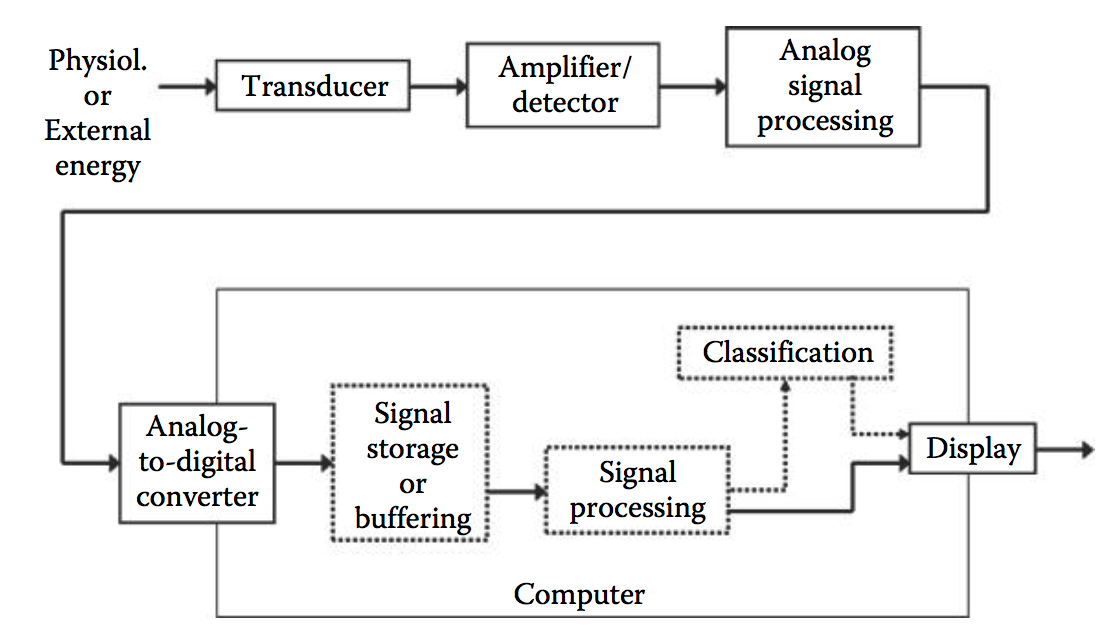
\includegraphics[width=0.8\textwidth]{signal-pipeline.png}
    \caption{Representación esquemática de las etapas del procesamiento de las bioseñales \cite{biosignal-book}.}
	\label{fig:signal-pipeline}
\end{figure}

\subsection{Obtención de la Señal Física}

Esta es la primer etapa en el procesamiento de bioseñales. Se debe obtener la señal de algún sensor. Puede ser un electrodo, un fotodetector, entre otros. La  señal viene en forma de energía. Dicha energía puede ser generada por el proceso en si (por ejemplo la actividad eléctrica producida por los músuclos), puede ser energía indirectamente relacionada al proceso o puede ser producida por una fuente externa \cite{biosignal-book}.

\subsection{Utilización de un Transductor}

Un transductor es un dispositivo que convierte energía de un tipo a otro. El propósito aquí es transferir información, no transformar energía. Se convierte la energía a energía eléctrica. Por lo general, la salida de un transductor de un biosensor es voltaje. En la figura \ref{fig:biotransducer} se puede observar una representación de un transductor. El trandsuctor es el elemento más crítico en el sistema ya que es la interfaz entre el sujeto y el resto del sistema. Este determina que tan invasivo es un dispositivo. Luego de pasar por el transductor, se utiliza un amplificador o detector \cite{biosignal-book}.

\begin{figure}[H]
	\centering
    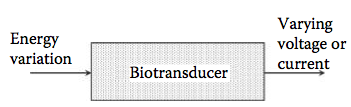
\includegraphics[width=0.8\textwidth]{biotransducer.png}
    \caption{Representación de un transductor utilizado en biosensores \cite{biosignal-book}.}
	\label{fig:biotransducer}
\end{figure}

\subsection{Procesamiento de la Señal Analógica}

La mayoría de los sensores procesan la señal analógica obtenida del transductor. El procesamiento más común es restringir el rango de frecuencias o ancho de banda utilizando filtros analógicos. Los filtros analógicos son dispositivos electrónicos que remueven un determinado rango de frecuencias. El filtrado es usualmente quien establece el ancho de banda de todo el sistema. La ganancia de un filtro es la relación entre la amplitud de la señal de salida y la amplitud de la señal de entrada define como:

$$ \textrm{Ganancia} (f) = \frac{\textrm{Valores de salida} (f)}{\textrm{Valores de entrada} (f)}  $$

Los filtros más comunes pueden observarse en al figura \ref{fig:filters} y son: 

\begin{itemize}
\item \textbf{Pasa bajos:} Atenúa las frecuencias superiores a un determinado valor. 
\item \textbf{Pasa altos:} Atenúa las frecuencias inferiores a un determinado valor. 
\item \textbf{Pasa bandas:} Atenúa las frecuencias fuera de un determinado intervalo.
\item \textbf{Supresión de bandas:} Atenúa las frecuencias dentro de un determinado intervalo \cite{biosignal-book}.

\end{itemize}

\begin{figure}[H]
	\centering
    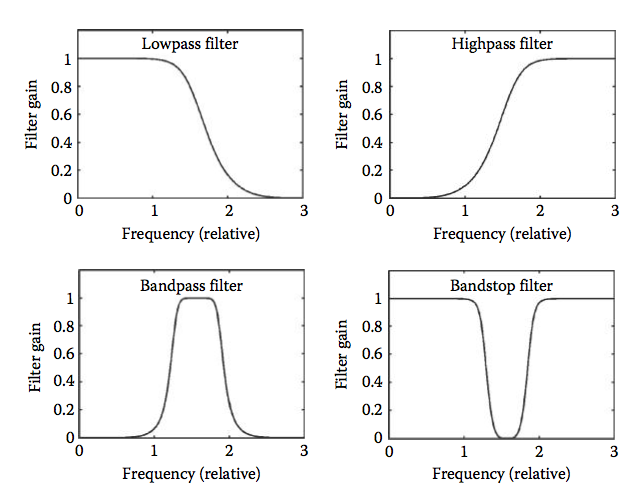
\includegraphics[width=0.8\textwidth]{filters.png}
    \caption{Influencia en la frecuencia de los filros básicos \cite{biosignal-book}.}
	\label{fig:filters}
\end{figure}

\subsection{Digitalización}

Todas las bioseñales son analógicas. Por este motivo, deben ser digitalizadas para poder ser utilizadas por una computadora. Este proceso ocurre en el dispositivo. Cuenta con un componente electrónico que convierte un voltaje analógico en número digital equivalente. Una onda continua ($ x(t) $) se convierte en una onda discreta ($x[t]$), una función de números reales que son definidos como enteros en puntos discretos en el tiempo. Estos números se conocen como muestras y los puntos discretos en el tiempo son usualmente tomados en intervalos regulares ($T$), también conocida como frecuencia de muestreo:

$$ f_{s} = \frac{1}{T_{s}}\, Hz $$

Entonces, la señal analógica es segmentada en varias partes para que pueda caber en la memoria de una computadora. Este concepto se conoce como ventana \cite{biosignal-book}. En la figura \ref{fig:digitalization} se puede observar el resultado digitalizar una señal continua.

\begin{figure}[H]
	\centering
    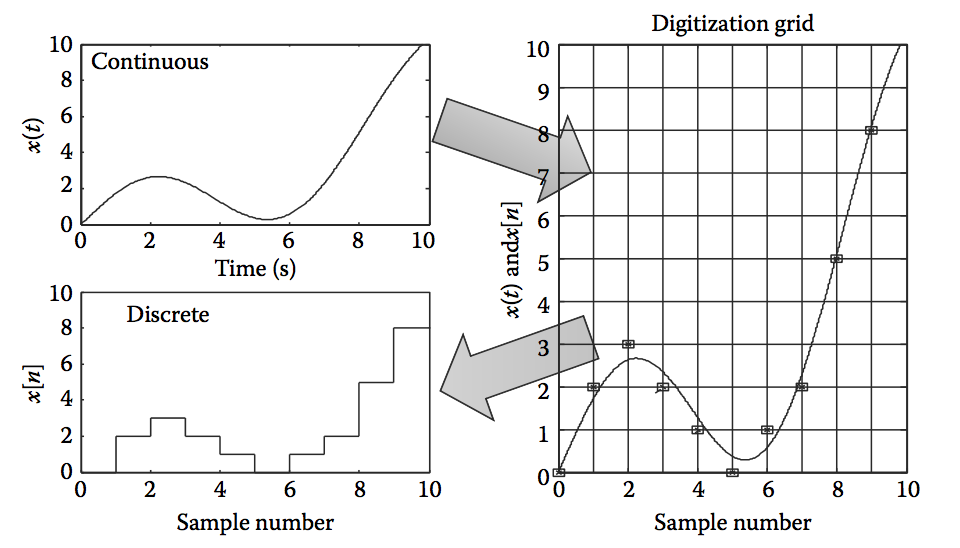
\includegraphics[width=0.8\textwidth]{digitalization.png}
    \caption{Digitalizar una señal continua, esquina superior izquierda, requiere partir la señal en tiempo y amplitud, lado derecho. El resultado es una serie de números disgretos que se aproximan a la señal, esquina inferior izquierda.  \cite{biosignal-book}.}
	\label{fig:digitalization}
\end{figure}

Digitalizar una señal implica segmentar la amplitud y el tiempo. Resulta evidente que la señal digitalizada obtenida no es igual a la analógica. El grado de aproximación de la señal digital a la analógica depende de la segmentación realizada. Como se mencionó, se segmentan las siguientes dos componentes:

\begin{itemize}
\item \textbf{Amplitud:} También se conoce como cuantificación. El grado de aproximación en este caso depende de la cantidad de valores distintos que son utilizados para representar la señal, es decir, la cantidad de bits utilizados. El nivel de cuantificación ($q$) se define como el tamaño del segmento de amplitud . El efecto de la cuantificación es la adición de ruido y este es determinado por $q$. En la figura \ref{fig:quantization} se puede observar el ruido añadido por la cuantificación. Por lo general los conversores usan $8$, $12$ y $16$ bits de salida. Pues la mayoría de las señales, no cuentan con una relación señal-ruido lo suficientemente elevada como para utilizar una resolución mayor.
\item \textbf{Tiempo:} Se refiere al muestreo. El criterio de \emph{Nyquist} establece que la frecuencia máxima (frecuencia de \emph{Nyquist}) obtenida es la mitad que la frecuencia de muestreo. El teorema de \emph{Shannon-Nyquist} establece que para poder recuperar la señal analógica a partir de la señal digital, se debe muestrear al doble que la máxima frecuencia contenida en la señal original, es decir, $ f_{s} > 2\, f_{max} $. Utilizar frecuencias de muestro más altas es innecesario e implica tener que guardar más información y tener que procesarla a una velocidad mayor \cite{biosignal-book}.  
\end{itemize}

\begin{figure}[H]
	\centering
    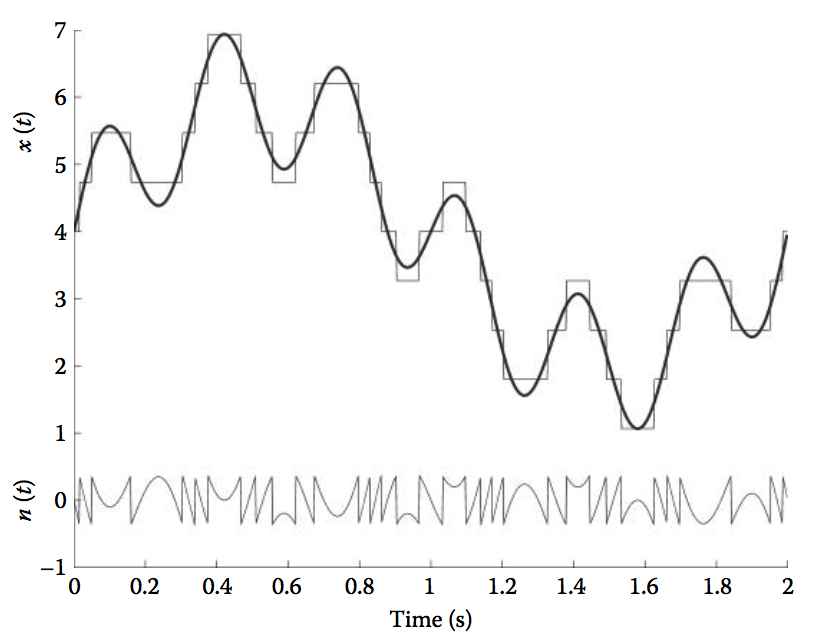
\includegraphics[width=0.8\textwidth]{quantization.png}
    \caption{El efecto de la cuantificación de la señal original puede verse como ruido añadido \cite{biosignal-book}.}
	\label{fig:quantization}
\end{figure}

\subsection{Transmisión de la Señal}\

Luego de digitalizar la señal, el dispositvo puede transmitirla hacia alguna computadora. Algunos dispositivos la utilizan directamente y no necesitan transmitirla. La transmisión puede tomar muchas formas. La señal puede ser transmitida por puerto serie, por USB, por \emph{bluetooth}, por \emph{wi-fi}, entre otros. El protocolo que se utilice para transmitir la señal depende del medio y es decisión del fabricante cuál utilizar. Por ejemplo si es un puerto serie, se transfiere bit a  bit. Luego, en la computadora debe haber un controlador que pueda recibir esta información transmitida.

\subsection{Procesamiento de la Señal Digital}

Como se mencionó anteriormente, la señal digital puede presentar ruido que se genera al digitalizarla. En algunos casos, hay que aplicar filtros para reducir el ruido. Existen diversos filtros. Uno de ellos es el filtro \emph{Gaussiano}. Dicho filtro suaviza la señal por lo que elimina los picos que se pudieran haber introducido.. Además, el filtro \emph{Gaussiano}, a diferencia de otros filtros, no elimina las altas frecuencias completamente. El filtro \emph{Gaussiano} se aplica haciendo una convolución de la señal con la siguiente función:
$$ g(x) = \frac{1}{\sqrt{2 * \pi} * \sigma } * e^{-\frac{x^{2}}{2 * \sigma^{2}}} $$

Muchas veces las señales pueden tener una cierta tendencia. Es decir, se encuentran desfasadas. Para compensar esta tendencia, se utiliza una técnica conocida como \emph{detrending}. Esta consiste en eliminar dicha tendencia.  La forma más simple de realizar \emph{detrending} es calcular la media del sensor y restarla a cada valor. Existen otros algoritmos más complejos de \emph{detrending} pero estos escapan al foco de este trabajo.

Una vez que se redujo el ruido, se pueden aplicar otros filtros o continuar. Como se mencionó anteriormente muchos sensores tienen como salida el nivel de potencial eléctrico medidas en $\mu V$ (microvoltios). Esta información sin ningún tipo de procesamiento no es útil. Dependiendo de que se quiera detectar se pueden realizar distintas operaciones. Una de ellas, es la búsqueda de picos. La primera derivada de un pico tiene un cruce descendente igual a cero en su máximo. Por ello, lo que se hace es primero suavizar la señal para eliminar ruido y luego se calculan las derivadas cruzadas. Luego, si la pendiente excede un umbral, significa que se ha encontrado un cero \cite{peak-finding}. Estos picos encontrados representan distintas cosas dependiendo el sensor utilizado. Por ejemplo, al utilizar un EMG, puede significar un impuslo de fuerza. En un EEG, puede significar un pestañeo.

Otro procesamiento que se le puede aplicar es la transformada discreta de \emph{Fourier}. La transformada de \emph{Fourier} transforma una función que se encuentra en el dominio del tiempo a una función que se encuentra en el dominio de la frecuencia. La transformada de \emph{Fourier} se define de la siguiente manera:

$$ x_{k} = \sum_{n=0}^{N-1} x_{n}e^{-\frac{2 \pi i}{N}kn} \qquad k = 0,\hdots, N - 1 $$

Computar la Transformada de \emph{fourier} tiene un costo computacional alto. Por este motivo, generalmente, se calcula la Transformada Rápida de \emph{Fourier} (\emph{FFT} por sus siglas en inglés). Esta es una aproximación a la Transformada de \emph{Fourier} y tiene un costo computacional menor. Para aplicar la \emph{FFT} se acumulan valores durante un período de tiempo. Esto se conoce como ventana. A esta ventana, se le puede aplicar una función de ventana. Una función de ventana es una función matemática en la cual el resultado es $0$ si los valores se encuentran fuera de un determinado intervalo y distinto de $0$ si se encuentran dentro de él. 

Una vez que la función se encuentra en el dominio de la frecuencia, se puede proceder con el procesamiento. Se selecciona el rango de frecuencias de interés y se le puede aplicar un filtro pasa banda, que deja pasar un determinado rango de frecuencias de una señal y atenúa el resto. Luego de aplicar el filtro pasa banda, se cuenta con las frecuencias de interés y se continúa con el procesamiento. Una alternativa es calcular la Densidad Espectral de Potencia (DEP). Esta se define como:

$$ P = \int_{-\infty}^{+\infty} S_{xx} (f) df \qquad  \textrm{donde,}$$

$$ S_{xx} = |X(f)|^{2} \qquad \textbf{y} \qquad X(f) \textrm{ es la Transformada de \emph{Fourier}} $$

Esta potencia puede ser utilizada luego como una característica de interés pero esto discutirá más adelante. Otra alternativa  es, por ejemplo, calcular el promedio de las frecuencias. Las posibilidades aquí son muchas y dependen de lo que se esté buscando.

\section{Extracción de Características de Interés y Clasificación}

Cuando se cuenta con la señal procesada, se puede utilizar directamente con reglas simples como utilizar un umbral. Este es el caso en el que se estén buscando picos. Si se buscan patrones más complejos, hay que utilizar reconocimiento de patrones. El reconocimiento de patrones tiene dos pasos principales:

\begin{itemize}
  \item \textbf{Extracción de características:} Esta etapa consiste en elegir características de la señal que sean relevantes al estado que se quiere clasificar. Por lo general estás características se colocan en un vector conocido como vector de características. El extractor utiliza como entrada una o más señales y las transforma en características útiles. Las características pueden ser por ejemplo ciertas bandas de frecuencia, calcular la DEP sobre una determinada banda de frecuencias, el valor de las derivadas en un instante del tiempo, entre otros. 
  \item \textbf{Clasificación:} En este paso se le asigna una clase a un conjunto de características (vector de características) extraído de la señal. Aquí se utilizan algoritmos de aprendizaje automático. Existen diversos algoritmos de clasificación, por ejemplo análisis discriminante lineal, árbol de decisión, clasificador bayesiano, entre otros \cite{eeg-tutorial}. También existen clasificadores más complejos como la utilización de redes neuronales.
\end{itemize}

Utilizar aprendizaje automático consiste en dos etapas:

\begin{itemize}
	\item \textbf{Calibración:} Consiste en adquirir la señal de entrenamiento, optimizar las características y entrenar el clasificador. Es decir, consiste en la acumulación de datos de entrenamiento que luego son enviados al clasificador.
	\item \textbf{Uso:} Consiste en usar el modelo (características y clasificador) obtenido durante la calibración para poder reconocer el estado del usuario \cite{eeg-tutorial}. 
\end{itemize}

En el caso de utilizar un EEG para detectar si el usuario tiene los ojos cerrados, en la etapa de calibración se obtienen los datos y extraen las características deseadas y se entrena al clasificador indicando a que estado (ojos abiertos o cerrados) corresponde cada dato. Luego, en la etapa de uso, se extraen las características de la señal del usuario y se envían al clasificador para que indique en que estado se encuentra.

\begin{figure}[H]
	\centering
    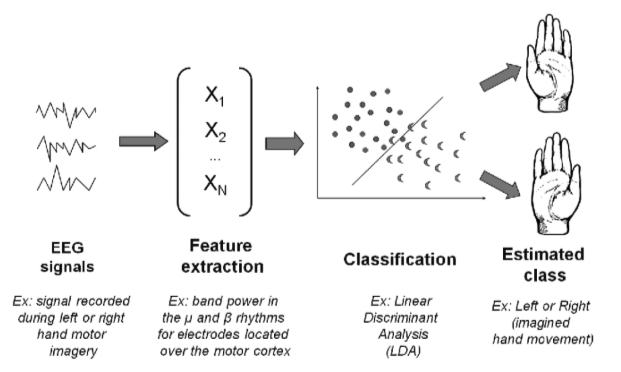
\includegraphics[width=0.8\textwidth]{eeg-pipeline.png}
    \caption{Ejemplo de las etapas por la que pasaría el procesamiento de una señal EEG \cite{eeg-tutorial}}.
	\label{fig:eeg-pipeline}
\end{figure}

En la figura \ref{fig:eeg-pipeline} se puede observar lo descripto anteriormente. Primero, se reciben las señales. Luego, se extraen las características. En este caso se trata de frecuencias asociadas a la corteza motora. Una vez que el vector de características fue creado, se envía al clasificador (en este caso análisis de discriminante lineal). Finalmente, el clasificador determina a que clase pertenece cada vector. En este ejemplo, se intento determinar si el usuario imaginó mover la mano derecha o la izquierda. 

Para medir la precisión del clasificador se arma una matriz de confusión. Esta, es una matriz de dos dimensiones en la cuál una dimensión representa los valores actuales y otra los valores predecidos. Por ejemplo, si utilizamos el ejemplo de ojos cerrados o abiertos, la matriz se armaría de la siguiente manera:

\[
\textrm{Mat} = \begin{blockarray}{ccc}
& A & C \\
\begin{block}{c(cc)}
  A & x & y \\
  C & w & z \\
\end{block}
\end{blockarray}
 \]
 
 , donde $ A $ representa el estado de ojos abiertos y $ C $, el de ojos cerrados. La primera dimensión representa el valor obtenido y la segunda el valor predecido. Por lo tanto, $Mat_{0,0}$ representa los positivos verdaderos ($TP$) (las veces que acertó el clasificador cuando el usuario tenía los ojos abiertos), $Mat_{0,1}$ representa los falsos negativos ($FN$) (valores que el clasificador clasificó como $C$ pero en realidad eran $A$), $Mat_{1,0}$ representa los falsos positivos ($FP$) (valores que el clasificador clasificó como $A$ pero en realidad eran $C$), y $Mat_{1,1}$ representa los verdaderos negativos ($TN$) (valores que el clasificador clasificó como $C$ y realmente eran $C$). Utilizando esta matriz se puede obtener la precisión, la cuál se define de la siguiente manera:
 
$$ ACC = \frac{TP + TN}{P + N} $$ 
, donde $P =$ total de casos positivos y $ N =$ total de casos negativos. O simplemente:

$$ ACC = \frac{Mat_{0,0} + Mat_{1,1}}{Mat_{0,0} + Mat_{0,1} + Mat_{1,0} + Mat_{1,1}} $$ 

Los valores cercanos a $0.5$ implican que el clasificador es malo y es azar. Cuantos más cercano $1$, mejor el clasificador.

Para determinar que parámetros de ajuste son los mejores para un modelo se puede utilizar el método de validación cruzada. Este consiste en subdividir un conjuntos de datos en subconjuntos, utilizar uno de ellos como datos de predicción y el resto como datos de entrenamiento. Luego se validan los subconjuntos de entrenamiento contra el subconjunto de predicción y se toma la media. La validación cruzada más simple es el método de regresión. Aquí simplemente se dividen los datos de la muestra en dos particiones: una de entrenamiento y una de validación. Este método es rápido de computar pero el problema es que la evaluación puede depender en gran medida de como es la división entre datos de prueba y de entrenamiento. La varianza puede ser muy elevada. Una mejora a este método de validación cruzada de k iteraciones cruzadas. Este consiste en dividir los datos en $k$ subconjuntos y utilizar   $k$ veces regresión lineal. Cada iteración se elige un subconjunto como conjunto de validación y el resto son usados como conjuntos de entrenamiento. Luego se toma el promedio de todas las iteraciones \cite{cross-validation}.

\subsection{Salida}

Una vez que la señal fue procesada, la información obtenida esta lista para ser utilizada. La salida puede ser, por ejemplo, una API de una librería que le permite a un usuario acceder a la información de forma amigable o una visualización en la computadora.
 
\section{Electroencefalograma}

Un electroencefalograma detecta la actividad eléctrica del cerebro. Estos cuentan con una determinada cantidad de electrodos que miden el nivel de potencial eléctrico en $ \mu V$. Al utilizar uno de estos dispositivos, la señal que se obtiene es el nivel de potencial eléctrico en cada electrodo. Un electroencefalograma no sirve si no se le da alguna aplicación. Aquí aparece el concepto de Interfaz Cerebro-computora (también conocido por sus silgas en inglés como BCI). "BCI es un método de comunicación basado en la actividad neuronal generada por el cerebro...El objetivo de BCI no es determinar la intensión de una persona espíando su actividad neuronal, sino que es proveer un nuevo canal de salida para el cerebro que requiere una adaptación de control voluntaria por parte del usuario"\cite{neural-eng}.

Al aplicar la Transformada de \emph{Fourier} a la señal EEG, se obtienen distintas frecuencias. En EEG, dichas frecuencias se dividen en cinco bandas:

\begin{itemize}
 \item \textbf{\emph{Alfa} ($\alpha$):} $ 8 \, Hz \leq f \leq 13 \, Hz$. Las ondas \emph{Alfa} se suprimen cuando los ojos se encuentran abiertos y hay estimulación visual presente. Cuando los ojos se encuentran cerrados, estas aumentan.
 \item \textbf{\emph{Beta} ($\beta$):} $ 13 \, Hz \leq f \leq 30 \, Hz$. Las ondas \emph{Beta} se asocian la concentración.
 \item \textbf{\emph{Delta} ($\delta$):} $ 0.5 \, Hz \leq f \leq 4 \, Hz$. Estas ondas aparecen en etapas de sueño profundo.
 \item \textbf{\emph{Theta} ($\theta$):} $ 4 \, Hz \leq f \leq 8 \, Hz$. Las ondas \emph{Theta} aparecen en las primeras etapas de sueño.
 \item \textbf{\emph{Gamma} ($\gamma$):} $ 30 \, Hz \leq f \leq 60 \, Hz$. Algunos expertos consideran los valores de $\beta > 30 \, Hz $ como una quinta banda. \cite{neural-eng}.
\end{itemize}

\section{Electromiografía}

La electromiografía consiste en registrar la actividad eléctrica producida por los músculos del cuerpo. La actividad eléctrica surge cuando una unidad motora es activada por el sistema nervioso del cuerpo: una unidad motora consiste en una motor neurona, y todas las fibras musculas a la que esta conectada.  Cuando se activa la unidad motora, se genera un voltaje (llamado MUAP, sus siglas en inglés) y se contraen los músculos.  Entonces, la señal EMG consiste en medir la suma de varios MUAPs de uno o mas músculos específicos.

El rango de la amplitud de una señal EMG es de aproximadamente $0\ mV$ a $10\ mV$, y su frecuencia de $0\, Hz$ a $500\, Hz$.  Sin embargo, el rango dominante de energía de la señal es de los $50\, Hz$ a $150\, Hz$, el cual es el que se intenta medir en este proyecto.

\section{Pulsioximetría}

La pulsioximetría permite determinar el porcentaje de sangre arterial saturado con oxígeno. Esta técnica no es invasiva y se basa en medir la absorción de luz roja e infraroja que pasa por el oído o dedo de una persona \cite{spo2-1}. Se basa medir una señal llamada \emph{Fotopletismografía}, la cual es una medición óptica del cambio de volumen de sangre en las arterias. Estas son obtenidas irradiando dos longitudes de onda de luz distintas a través del tejido. Existen dos formas de leer la oxigenación en sangre: transmisión y reflexión de la luz. En transmisión, se envían haces de luz utilizando una luz LED y se utiliza un fotodetector del otro lado que detecta estos haces. En cambio, en reflexión, se coloca un fotodetector del mismo lado que la luz led y se detecta la reflexión de la luz \cite{spo2-2}.

El corazón bombea sangre a través de las arterias de forma continua. Este es conocido como el ciclo cardíaco. Este ciclo puede ser observado con un pulsioximetro ya que se generan variaciones de volumen en las arterias \cite{spo2-2}. En la figura \ref{fig:cardiac-cycle} se pueden observar los picos generados por el ciclo cardíaco. Dichos picos son utilizados para estimar el ritmo cardíaco. 

\begin{figure}[H]
	\centering
    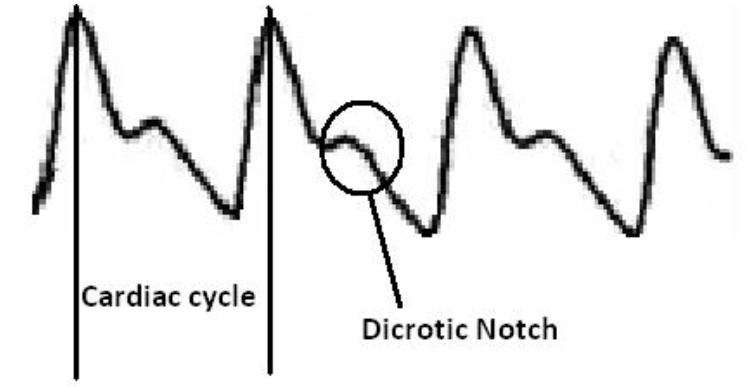
\includegraphics[width=0.8\textwidth]{cardiac-cycle.png}
    \caption{Ciclo cardíaco}.
	\label{fig:cardiac-cycle}
\end{figure}

Existen dos formas de calcular el ritmo cardíaco a partir de los picos:

\begin{itemize}
 \item \textbf{Promedio:} Se cuentan la cantidad de picos en un determinado tiempo y luego se utiliza la regla de tres simple. El problema es que este método no permite observar cambios en el tiempo y por lo tanto no representa verdaderamente la respuesta al ejercicio, el estrés y el ambiente.
 \item \textbf{Latido a latido:} Se mide el tiempo ($T$) entre dos picos consecutivos y luego se calcula usando la fórmula $60/T$ \cite{spo2-1}.
\end{itemize}

Se pueden combinar estas dos metodologías y promediar los últimos cuatro o seis resultados obtenidos \cite{spo2-1}.

Existen otras formas de monitorear el ritmo cardíaco como la electrocardiografía. Esta consiste en registrar la actividad eléctrica del corazón utilizando electrodos. 
